% Outline
% 
% Section 1
%   History of GeoSPARWL 1.0
% Section 2
%   motivation to update the spec
% Section 3
%   GeoSPARQL 1.1 additions
%       motivation, and expected use, of new spatial functions. In particular, why in GeoSPARQL when aggregations etc. can be performed elsewhere?
%       Spatial Measure
% Section 4
%       new profile preentation
%       new URI regimes etc
% Section 5
%       expected changed use modes
\documentclass[runningheads]{llncs}

\usepackage{graphicx}
\usepackage{todonotes}
\usepackage{listingsutf8}
\usepackage[hidelinks]{hyperref}
\usepackage{cleveref}

\renewcommand\UrlFont{\color{blue}\rmfamily}

\begin{document}

\title{GeoSPARQL 1.1: an almost decadal update to the most important geospatial LOD standard}
\titlerunning{GeoSPARQL 1.1}

\author{
    Nicholas J. Car\inst{1}\orcidID{0000-0002-8742-7730} \and \\
    Timo Homburg\inst{2}\orcidID{0000-0002-9499-5840} \and \\
    Simon J.D Cox\inst{3}\orcidID{0000-0002-3884-3420}
}

\authorrunning{Car N.J. et al.}

\institute{
    {
    SURROUND Australia Pty Ltd., Australia \&\\
    Australian National University, Australia\\
    \email{nicholas.car@surroundaustralia.com}\\
    \url{https://surroundaustralia.com}
    }
    \and
    {
        Mainz University Of Applied Sciences, Germany\\
        \email{timo.homburg@hs-mainz.de}
    }
    \and 
    {
        Commonwealth Scientific \& Industrial Research Organisation, Australia\\
        \email{simon.cox@csiro.au}
    }
}

\maketitle

\begin{abstract}
The Open Geospatial Consortium published the GeoSPARQL 1.0 standard in 2012 containing multiple 
parts that define ``SPARQL extension functions'', ``RIF rules'', ``an RDF/OWL ontology for 
information based on the General Feature Model'' and supporting vocabularies, all for Semantic 
Web spatial data.\\

In the 8+ years since its publication, GeoSPARQL has become the most important spatial Semantic 
Web standard, as judged by references to it in other Semantic Web standards and its wide use in 
Semantic Web data.\\

An update to the standard was proposed in 2019 to deliver GeoSPARQL 1.1 in 2021 with a charter to: 
handle outstanding change requests and source new ones from the GeoSPARQL user community as well 
to ``better present'' the standard, that is to better link all the standard’s parts and better 
document \& exemplify elements. Expected updates included possible alignments to other ontologies, 
possible handling of new spatial referencing systems, new geometry representations, and new artifact 
presentation.\\

In this paper, we will discuss the submitted change requests and resulting updates to the standard. 
We will also discuss the theory behind updates and our expectations for GeoSPARQL 1.1's use.

\keywords{GeoSPARQL  \and GeoSPARQL 1.1 \and spatial \and geospatial \and Semantic Web \and RDF \and OWL \and OGC \and Open Geospatial Consortuim \and standard.}
\end{abstract}

\section{Introduction}\label{sec:introduction}
The GeoSPARQL standard, first issues in 2021 by the Open Geospatial Consortium (OGC)\footnote{\url{https://www.ogc.org}} 
is one of, if not the most\footnote{It is hard to calculate use but references to GeoSPARQL in papers and other 
well-known standards, such as DCAT2 (\url{https://www.w3.org/TR/vocab-dcat/}) suggests this}, used 
\textit{Sematic Web} ontologies for representing spatial data.

The original GeoSPARQL release, which we refere to as GeoSPARQL 1.0, contained a \textit{specification} document,
a main ``GeoSPARQL'' ontology in an RDF file and a ``Simple Features Vocabulary'' ontology also in an RDF file. The 
``GeoSPARQL'' ontology content, as well as lists of geospatial functions that could be performed on RDF data via 
SPARQL\footnote{\url{https://www.w3.org/TR/sparql11-query/}} queries was defined in the specification document, as
were entailement rules and requirements \& abstract tests for testing ontology data and function implementations. 
Within the last few years, the function lists from the sepecification were extracted into a SKOS\footnote{\url{https://www.w3.org/TR/skos-reference/}}
vocabulary.


\section{Motivation to update GeoSPARQL}\label{sec:motivation}
Interest in updating GeoSPARQL had been captured\footnote{\href{https://www.w3.org/2015/spatial/wiki/Further_development_of_GeoSPARQL}{https://www.w3.org/2015/spatial/wiki/Further\_development\_of\_GeoSPARQL}}
 by the World Wide Web Consortium's (W3C) \textit{Spatial Data On The Web Working Group} (SDWWG)
when a large body of work was done on \textit{Semantic Web} spatial data around in approximately 2015 - 2017, but 
no updates to GeoSPARQL were ultimately made by that Working Group.

% Spatial Data On The Web Best Practices \cite{van2019best}

Recently, 2019, the OGC reconstituted a \textit{GeoSPARQL Standards Working Group} (SWG) to update GeoSPARQL. The general 
motivation for work within the area of GeoSPARQL, that of \textit{Semantic Web} spatial data, and a series of
fault fixes and proposed extensions to GeoSPARQL 1.0 are captured in an OGC White Paper \cite{geosparqlwhitepaper}. Some,
but not all, of the SDWWG's proposals are included in the White Paper with the different communities - W3C and OGC - 
naturally reflecting different desires.

The SWG's charter - it's final scope of work - is also published by the OGC \cite{abhayaratna2020ogc} and this guides 
the SWG's activities. Specific actions of the SWG and their staging are explained through the use of a publicly-available 
online task tracking system within the SWG's working online code repository\footnote{\url{https://github.com/opengeospatial/ogc-geosparql/projects/1}}.

At a high-level, proposed updates to GeoSPARQL by both the SDWWG and the SWG may be categorised as:

% Nick up to here

\begin{itemize}
    \item small geometry extensions, as predicted in GeoSPARQL 1.0
    \item class extensions to cater for spatial information in RDF/OWL with more fidelity
    \item 
\end{itemize}








\section{New features in GeoSPARQL 1.1}\label{sec:newfeatures}
One of the first actions undertaken by the SWG was to link the GeoSPARQL 1.0 elements through a \textit{profile} 
declaration, where a profile is a special type of \textit{specification}, as defined by \textit{The Profiles Vocabulary}\cite{atkinson_profiles_2020}. 
The specific motivation for this was the SWG's recognition that GeoSPARQL 1.0 consisted of multiple parts, not all
of which were easy to discover and, as a result, some GeoSPARQL users were unaware of some of the resources and some
resources were accidentally duplicated or partly re-implemented.

The profile declaration will be published by the OGC as a stand-alone resource sometime in mid-2021 along with some 
updated GeoSPARQL 1.0 resources. Currently, all of the elements of GeoSPARQL 1.0, including the profile declaration, 
can be found within the SWG's working online repository \footnote{\url{https://github.com/opengeospatial/ogc-geosparql}}.

% GeoSPARQL 1.1 includes non-breaking changes to the GeoSPARQL 1.0 standard.

\subsection{New geometry literals}\label{sec:literals}
GeoSPARQL 1.1 introduces three new literal types: A GeoJSON\cite{butler2016geojson} literal, a KML\cite{nolan2014keyhole} literal, and a DGGS\cite{sahr1998discrete} WKT Literal.
\small
\begin{lstlisting}[caption=GeoJSON literal example,label=lst:geojsonliteral,language=sql,frame=single,basicstyle=\ttfamily]
"{\"type\":\"Point\", \"coordinates\":[-83.38,33.95]}"
^^<http://www.opengis.net/ont/geosparql#geoJSONLiteral>
\end{lstlisting}
\normalsize
Since the GeoJSON and KML formats are restricted to be represented in the WGS84 coordinate system only, these restrictions also apply to GeoJSON and KML literals. The DGGS WKT literal  
\subsection{Spatial aggregate functions}\label{sec:spatialaggregate}
GeoSPARQL 1.1 includes new spatial aggregate functions, which allow for the quick aggregation of different geometry types. While spatial aggregate functions are the norm in many non-semantic geospatial databases such as POSTGIS or Oracle Spatial, at the time of defining the GeoSPARQL 1.0 standard, aggregate functions had not yet been introduced into the SPARQL standard since SPARQL 1.1 \cite{w3c_sparql_working_group_sparql_2013} was released about one year later. Spatial aggregate functions similar to traditional aggregate functions such as AVG,MAX, or MIN allow to aggregate results of geometry queries, e.g., to create the union out of a set of given geometry literal results. While calculating these aggregates may also be possible outside of the semantic database, the inclusion of the functions provides distinct advantages:
\begin{enumerate}
    \item No client-side library is needed to create an aggregated geometry result
    \item Fewer and more appropriate results can be returned using a spatial aggregate function (e.g., a single union geometry vs. a set of geometries for which to create union externally)
    \item Spatial aggregates from different SPARQL endpoints can easily be calculated using federated queries 
\end{enumerate}
GeoSPARQL 1.1 defines the aggregate functions \emph{geosf:boundingCircle}, calculating a bounding circle around a set of geometry, \emph{geosf:centroid} calculating the centroid of the set of geometries, \emph{geosf:concatLines} concatenating a set of linestrings that overlap, \emph{geosf:concaveHull} calculating the concave hull of a set of geometries and\emph{geosf:union}, calculating the union of a set of geometreis, in addition to the \emph{geosf:envelope} and \emph{geosf:convexHull} functions already defined in the GeoSPARQL 1.0 standard. Since SPARQL 1.1 these fucntions were also usable as aggregate functions.
Spatial aggregate function definitions are accompanied by the functions \href{http://www.opengis.net/def/function/geosparql/maxX}{\emph{geof:maxX}}, \href{http://www.opengis.net/def/function/geosparql/maxY}{\emph{geof:maxY}}, \href{http://www.opengis.net/def/function/geosparql/maxZ}{\emph{geof:maxZ}} and \href{http://www.opengis.net/def/function/geosparql/minX}{\emph{geof:minX}}, \href{http://www.opengis.net/def/function/geosparql/minY}{\emph{geof:minY}}, \href{http://www.opengis.net/def/function/geosparql/minZ}{\emph{geof:minZ}} which allow to retrieve the minimum and maximum coordinates of a geometry respectively.


\subsection{Extensions of the GeoSPARQL ontology}\label{sec:ontologyextensions}
GeoSPARQL 1.1 extends the GeoSPARQL ontology by adding a new class \href{http://www.opengis.net/ont/geosparql#SpatialMeasure}{geo:SpatialMeasure}. This class represents a measurement such as a volume, length, or area associated with a measurement amount and a measurement unit. It acts as a range of three newly defined properties \href{http://www.opengis.net/ont/geosparql#hasVolume}{geo:hasArea}, \href{http://www.opengis.net/ont/geosparql#hasLength}{geo:hasLength},
\href{http://www.opengis.net/ont/geosparql#hasVolume}{geo:hasVolume} which make these attributes of a geometry better accessible using SPARQL. Finally, GeoSPARQL 1.1 adds the \href{http://www.opengis.net/ont/geosparql#inCRS}{geo:inCRS} property, which allows querying the coordinate reference system of a given geometry without the need to analyze geometry literal serializations. The property allows for the definition of a CRS as a URI. It paves the way for a future definition of coordinate reference systems fully in RDF as anticipated for GeoSPARQL 2.0.
\todo[inline]{I created a graphic (geold\_ontology.graphml) containing geo:SpatialObject, geo:Feature, geo:SpatialMeasure using the yEd Editor (https://www.yworks.com/products/yed) . If you find it useful we can extend it. }
\begin{figure}[htb]
    \centering
    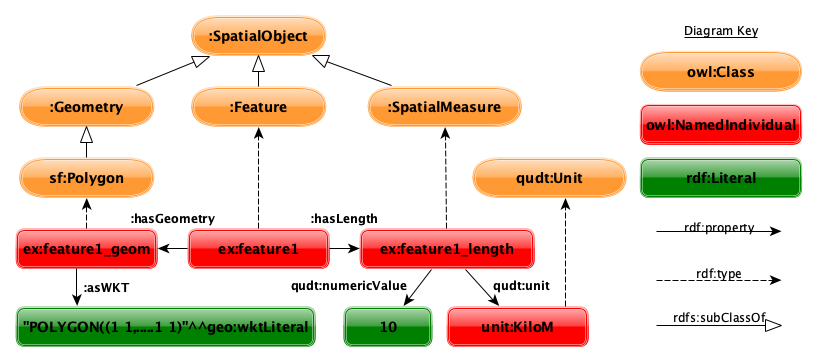
\includegraphics[width=\linewidth]{images/geold_ontology.png}
    \caption{GeoSPARQL 1.1 ontology including one example feature}
    \label{fig:geosparql11ontology}
\end{figure}


\section{Modernizing the documentation of GeoSPARQL}\label{sec:documentation}


\subsection{Profile}\label{sec:profile}


\section{Conclusions}\label{sec:conclusions}

\subsection{Future Work}\label{sec:futurework}
GeoSPARQL 1.2, GeoSPARQL 2.0?
\begin{itemize}
    \item GeoSPARQL extension ontologies: CRS systems
    \item GeoSPARQL 1.2: More literals?
    \item GeoSPARQL 2.0: Full featured support for 3D, simple features functions, coverages?
\end{itemize}
%   History of GeoSPARWL 1.0
% Section 2
%   motivation to update the spec
% Section 3
%   GeoSPARQL 1.1 additions
%       motivation, and expected use, of new spatial functions. In particular, why in GeoSPARQL when aggregations etc. can be performed elsewhere?
%       Spatial Measure
% Section 4
%       new profile preentation
%       new URI regimes etc
% Section 5
%       expected changed use modes


%
% ---- Bibliography ----
%
% BibTeX users should specify bibliography style 'splncs04'.
% References will then be sorted and formatted in the correct style.
%
\bibliographystyle{splncs04}
\bibliography{GeoSPARQL}
%
% \begin{thebibliography}{8}
% \bibitem{ref_article1}
% Author, F.: Article title. Journal \textbf{2}(5), 99--110 (2016)

% \bibitem{ref_lncs1}
% Author, F., Author, S.: Title of a proceedings paper. In: Editor,
% F., Editor, S. (eds.) CONFERENCE 2016, LNCS, vol. 9999, pp. 1--13.
% Springer, Heidelberg (2016). \doi{10.10007/1234567890}

% \bibitem{ref_book1}
% Author, F., Author, S., Author, T.: Book title. 2nd edn. Publisher,
% Location (1999)

% \bibitem{ref_proc1}
% Author, A.-B.: Contribution title. In: 9th International Proceedings
% on Proceedings, pp. 1--2. Publisher, Location (2010)

% \bibitem{ref_url1}
% LNCS Homepage, \url{http://www.springer.com/lncs}. Last accessed 4
% Oct 2017
% \end{thebibliography}
\end{document}
